\documentclass[11pt]{article}

\usepackage{graphicx}
\usepackage{geometry}
\usepackage{tikz-cd}
\usepackage{amsmath}
\usepackage{amssymb}
\usepackage{authblk}

\usepackage{listings}
\usepackage{xcolor}

\definecolor{codegreen}{rgb}{0,0.6,0}
\definecolor{codegray}{rgb}{0.5,0.5,0.5}
\definecolor{codepurple}{rgb}{0.58,0,0.82}
\definecolor{backcolour}{rgb}{0.95,0.95,0.92}

\lstdefinestyle{mystyle}{
    backgroundcolor=\color{backcolour},   
    commentstyle=\color{codegreen},
    keywordstyle=\color{magenta},
    numberstyle=\tiny\color{codegray},
    stringstyle=\color{codepurple},
    basicstyle=\ttfamily\footnotesize,
    breakatwhitespace=false,         
    breaklines=true,                 
    captionpos=b,                    
    keepspaces=true,                 
    numbers=left,                    
    numbersep=5pt,                  
    showspaces=false,                
    showstringspaces=false,
    showtabs=false,                  
    tabsize=2
}

\lstset{style=mystyle}



\geometry{a4paper,scale=0.8}
\title{Lab 1: Modeling Packet Losses}
\author{Zhipeng Ye}
\affil{Department of Electrical and Electronic Engineering \\Xi’an Jiaotong-Liverpool University}
\begin{document}

\maketitle
    \section{Hidden Markov Model}
    \paragraph{}
    Gilbert-Elliott Model is packet loss model which is based on two-state Hidden Markov Model.
    In other words, Gilbert-Elliott Model is a simply version of Hidden Markov Model. 
    Therefore, It's necessary to learn more about Hidden Markov Model to understand Gilbert-Elliott Model completely.
    \begin{figure}[ht]
        \centering
        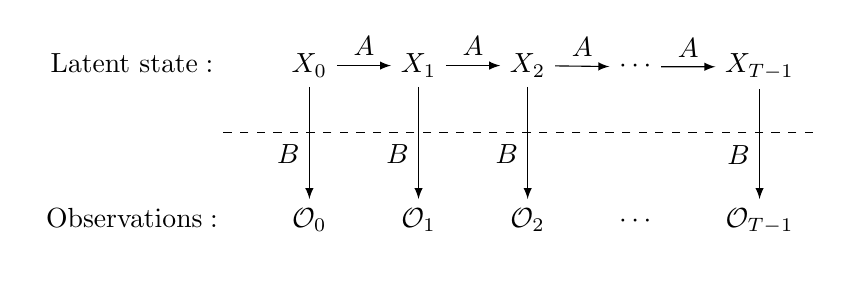
\begin{tikzpicture}
            \matrix[matrix of math nodes,column sep=2em,row sep=4em] (m) {
            \text{Latent state}: &
             X_0 & X_1 & X_2 & \cdots & X_{T-1}\\
            \text{Observations}: & 
             \mathcal{O}_0 & \mathcal{O}_1 & \mathcal{O}_2 & \cdots & \mathcal{O}_{T-1}\\
            };
            \foreach \X in {2,3,4,5}
            {\draw[-latex] (m-1-\X) -- (m-1-\the\numexpr\X+1) node[midway,above]{$A$};
            \ifnum\X=5
            \draw[-latex] (m-1-6) -- (m-2-6) node[pos=0.6,left]{$B$};
            \else
            \draw[-latex] (m-1-\X) -- (m-2-\X) node[pos=0.6,left]{$B$};
            \fi}
            \draw[dashed] ([yshift=1ex]m.east) -- ([yshift=1ex]m.east-|m-1-1.east);
            \end{tikzpicture}
        \caption{Hidden Markov Model}
        \label{fig:ch5:jointentropy}
    \end{figure}
    \paragraph{}
    Hidden Markov Model introduce two random variable - Latent state and Observations. Latent state is a variable that we can't see.
    Observations is a variable that we can observe at the experiment.
    Furtheremore, HMM also has three parameters - initial probability vector $\pi$, transition probability matrix $A$,
    emission probability matrix $B$. So if we can compute three parameters $\{A,B,\pi\}$, we will reconstruct HMM.
    Researchers have developed numerous approaches to estimate parameters of Hidden Markov Model (HMM) such as Forward/Backward Algorithm.
    \paragraph{}
    Markov Model simplifies the Hidden Markov Model (HMM). It only uses two parameters $\{A,\pi\}$ and removes the Latent state. Maximum likelihood estimation (MLE) is a good way to 
    estimate these parameters. The relationship between Hidden Markov Model and Markov Model is similar to the relation between Gilbert-Elliott Model (GM) and Simple Gilbert-Elliott Model (SGM). Section two of this article will demonstrate the reason. 
    \section{Gilbert-Elliott Model}
    \paragraph{}Gilbert-Elliott Model resembles Hidden Markov Model. To be specific, Gilbert-Elliott Model has two state - $\{Good, Bad\}$ , transition matrix $\boldsymbol{P}=\left[\begin{array}{cc}(1-p) & q \\ p & (1-q)\end{array}\right]$ and emission probability vector $\left[\begin{array}{cc}1-k&1-h\end{array}\right]^T$.
    \paragraph{}
        \begin{figure}[ht]
        \centering
        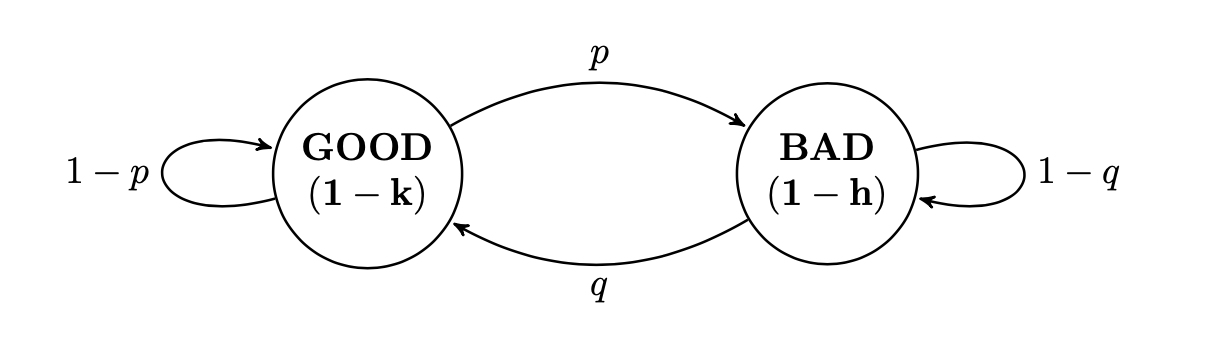
\includegraphics[scale=0.5]{figure1.png}
        \caption{Gilbert-Elliott Model}
        \label{fig:label}
    \end{figure}
    Furtheremore, we can obtain the other parameters of Gilbert-Elliott Model such as the steady state probability vector $\pi$, packet loss probability $p_L$ and the probability distribution of loss run length $p_k$.
    The steady state probability vector $\boldsymbol \pi$ satisfies the following conditions:
    \begin{equation}
        \boldsymbol{\pi} = \boldsymbol{P}\boldsymbol{\pi}, \boldsymbol{1}^T\boldsymbol{\pi}
    \end{equation}
    where 
    \begin{equation}
        \boldsymbol{\pi} = \left[
        \begin{array}{c}
            \pi_{G} \\ \pi_{B}
        \end{array}        
        \right]
    \end{equation}
    The steady state probabilities exist for $0<p$, $q<1$ and are given by 
    \begin{equation}
        \pi_G = \frac{q}{p+q},\pi_B = \frac{p}{p+q}
    \end{equation}
    From equation (3), we can get packet loss probability $p_L$ as follows:
    \begin{equation}
        p_L = (1-k)\pi_G + (1-h)\pi_B
    \end{equation}
    The special cases of $k=1$ and $k=1,h=0$ are called a Gilbert Model (GM) and a simple Gilbert Model
(SGM), respectively.
Note that in case of the SGM, the probability distribution of loss run length has a geometric distribution,
i.e.,
\begin{equation}
    p_{k} \triangleq \text { Prob }\{\text { loss run length }=k\}=q(1-q)^{k-1} \text { for } k=1,2, \ldots, \infty
\end{equation}
\section{Estimation of parameters}
\subsection{Simple Gilbert Model (SGM)}
\paragraph{}
Because $0,1$ represent $\{Good,Bad\}$ respectively. The probabilities from \emph{Good to Bad} is equal to $P(1|0)$ and 
the probabilities from \emph{Bad to Good} is equal to $P(0|1)$. According to \emph{Bayes theorem}, 
\begin{equation}
    \begin{array}{lr}
    p = P(1|0) = \frac{P(01)}{P(0)} = \frac{n_{01}}{n_0} &\\ \\
    q = P(0|1) = \frac{P(10)}{P(1)} = \frac{n_{10}}{n_1}
    \end{array}
\end{equation}
$n_{10}$ means the times 0 follows 1 . $n_{01}$ means the times 1 follows 0. $n_0$ represents the times of 0. $n_1$ represents the times of 1.
\subsection{Gilbert Model (GM)}
Gilbert applied a method to decide the parameters of GM \cite{Gilbert Model}.
Firstly, the parameters of ${p,q,h}$ can be estimated from another parameters of ${a,b,c}$. 
The expression equation of ${a,b,c}$ is as follow:
\begin{equation}
    a=P(1), b=P(1 | 1), c=\frac{P(111)}{P(101)+P(111)}
\end{equation}
Finally, we can get parameters of Gilbert Model by the following relation between these variables.
\begin{equation}
    1-q=\frac{a c-b^{2}}{2 a c-b(a+c)}, h=1-\frac{b}{1-q}, p=\frac{a q}{1-h-a}
\end{equation}

\section{Experiment Task}
In this experiment, we simulate the Simple Gilbert Model (SGM) and Gilbert Model (GM) separately.
\subsection{Simple Gilbert Model (SGM)}
\subsubsection{Construct model}
The script and detailed comments for Constructing Simple Gilbert Model is attached at the appendix \ref{CSGM}.
The main implement is here.
\begin{verbatim}
# main loop
for i in range(len):
    # if the random sequence is large than the transition probability
    # we must change the state for example 0 -> 1 or 1 -> 0
    if statechange[i] > tr[state, state]:
        # transition into the other state
        state ^= 1
    # add a binary value to output
    seq[i] = state
\end{verbatim}
As we can see from the code segment, if the sequence[i] is large than the transition probability, the start will flip from $0$ to $1$ or from $1$ to $0$.
\subsubsection{Estimate model parameters}
To determine the parameters of $p,q$, I write the script to count the number of times where binary sequence occurs.


\subsubsection{Comparison and discussion}

\subsection{Gilbert Model (GM)}
\subsubsection{Construct model}

\subsubsection{Estimate model parameters}


\subsubsection{Comparison and discussion}
\newpage
\appendix{Detailed Python Script Appendix}
\section{Construct Simple Gilbert Model (SGM)} \label{CSGM}
\begin{lstlisting}[language=Python]
    #!/usr/bin/env python
# -*- coding: utf-8 -*-
##
# @file     sgm_generate.py
# @author   Kyeong Soo (Joseph) Kim <kyeongsoo.kim@gmail.com>
# @date     2020-03-25
#
# @brief    A function for generating loss pattern based on simple Guilbert model.
#

import numpy as np
import sys


def sgm_generate(len, tr):
    """
    Generates a binary sequence of 0 (GOOD) and 1 (BAD) of length
    len from an SGM specified by a 2x2 transition probability matrix
    tr; tr[i, j] is the probability of transition from state i to
    state j.

    This function always starts the model in GOOD (0) state.

    Examples:

    import numpy as np

    tr = np.array([[0.95, 0.10],
                   [0.05, 0.90]])
    seq = sgm_generate(100, tr)
    """

    seq = np.zeros(len)

    # tr must be 2x2 matrix
    tr = np.asarray(tr)  # make sure seq is numpy 2D array
    if tr.shape != (2, 2):
        sys.exit("size of transition matrix is not 2x2")

    # create a random sequence for state changes
    statechange = np.random.rand(len)

    # Assume that we start in GOOD state (0).
    state = 0

    # main loop
    for i in range(len):
        # if the random sequence is large than the transition probability
        # we must change the state for example 0 -> 1 or 1 -> 0
        if statechange[i] > tr[state, state]:
            # transition into the other state
            state ^= 1
        # add a binary value to output
        seq[i] = state

    return seq


if __name__ == "__main__":
    import argparse

    parser = argparse.ArgumentParser()
    parser.add_argument(
        "-L",
        "--length",
        help="the length of the loss pattern to be generated; default is 10",
        default=10,
        type=int)
    parser.add_argument(
        "-T",
        "--transition",
        help="transition matrix in row-major order; default is \"0.95,0.10,0.05,0.90\"",
        default="0.95,0.10,0.05,0.90",
        type=str)
    args = parser.parse_args()
    len = args.length
    tr = np.reshape(np.fromstring(args.transition, sep=','), (2, 2))
    print(sgm_generate(len, tr))

\end{lstlisting}

\newpage
\begin{thebibliography}{9}
\bibitem{Gilbert Model} 
E. N. Gilbert, “Capacity of a burst-noise channel,” Bell System Technical Journal, vol. 39, no. 5, pp. 1253–1265, Sep. 1960.
\end{thebibliography}
\end{document}
